\documentclass[12pt]{article}
%\usepackage[utf8]{inputenc}
%\documentclass[UTF8]{ctexart}
%\usepackage[UTF8, heading = false, scheme = plain]{ctex}
\usepackage{geometry}
%geometry{a4paper,scale=0.9}
\geometry{a4paper,left=1cm,right=1cm,top=1cm,bottom=2cm}
\usepackage{amsfonts}
\usepackage{color}
\usepackage{url}
%\usepackage{biblatex}
\usepackage{amsmath}
\usepackage{amssymb}
\usepackage{latexsym}
\usepackage{cite}
%\addbibresource{ref.bib}
%\bibliography{ref.bib}
\usepackage{caption}
\usepackage{graphicx, subfig}
\usepackage{float}
%\usepackage[fontset=ubuntu]{ctex}
%\usepackage{fontspec}
\usepackage{xeCJK}
%\usepackage[colorlinks,
%anchorcolor=black,
%citecolor=black]{hyperref}
%\setmainfont{SimSun}
\usepackage[section]{placeins}
\usepackage{enumitem}
\usepackage{framed}
\usepackage[framemethod=TikZ]{mdframed}
\usepackage{indentfirst}
\usepackage{setspace}%使用间距宏包
\linespread{1.5}
%\title{预备知识}
%\author{leolinuxer }
%\date{June 2020}

\title{最小二乘法\cite{Understand_Least_Square_Method}}
\author{leolinuxer}
%\date{June 2020}

\begin{document}
\maketitle

\section{举例}
有五把尺子测量同一个长度,得到的数据会有细微的差别,一般来说,我们都是使用\textbf{算数平均值}作为最终结果的;

可是,深入思考一下这个问题,为什么要用算数平均值呢?用调和平均数行不行?用中位数行不行?用几何平均数行不行?

\section{最小二乘法}
换一种思路来思考刚才的问题。
首先,把测试得到的值画在笛卡尔坐标系中,分别记作$y_i$;然后,把要猜测的线段长度的真实值用平行于横轴的直线来表示(因为是猜测的,所以用虚线来画),记作$y$;每个点都向$y$做垂线,垂线的长度就是$|y-y_i|$,也可以理解为测量值和真实值之间的误差,如下图所示:
\begin{figure}[H]
  \centering
  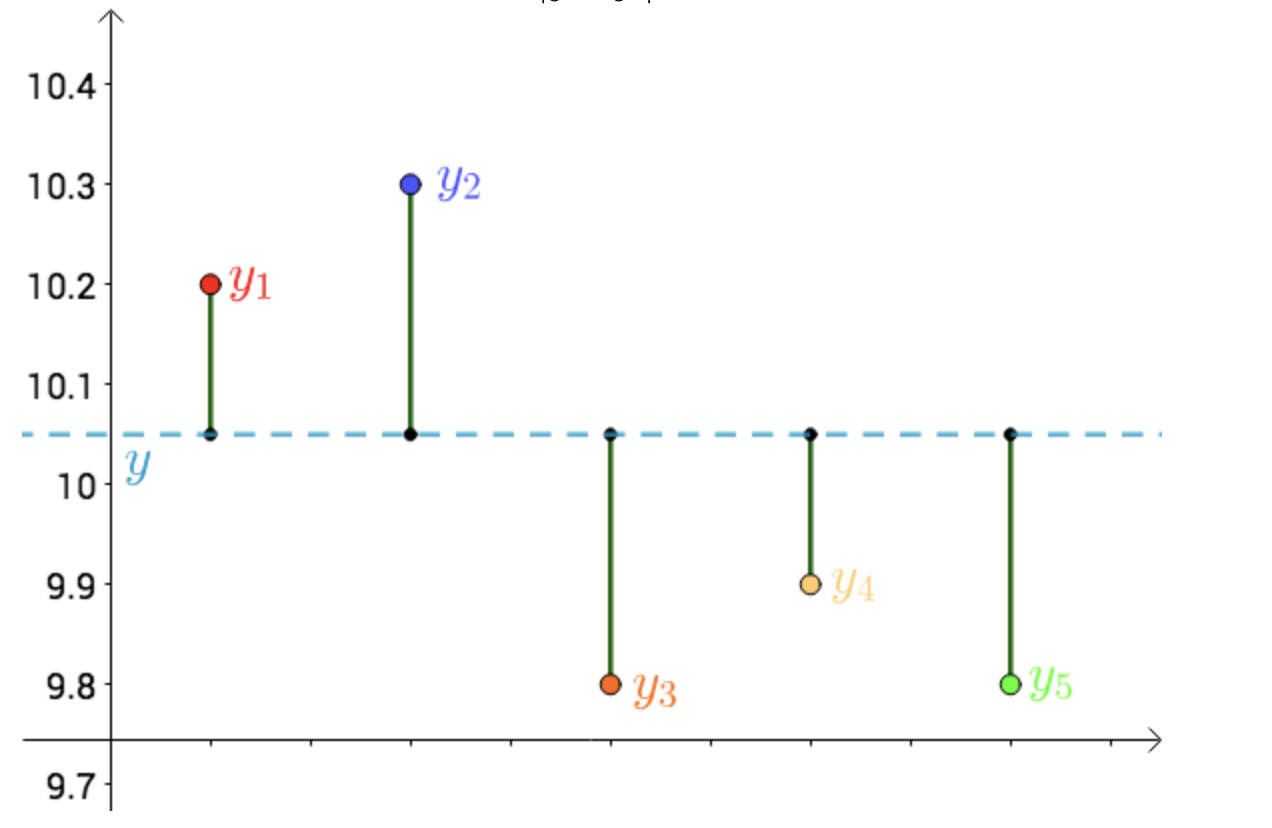
\includegraphics[width=.8\textwidth]{fig/LeastSquareMethod_Example.png} 
\end{figure}

因为误差是长度,还要取绝对值,计算起来麻烦,就干脆用平方来代表误差:
$|y-y_i|\to (y-y_i)^2$

总的误差的平方就是:
$$
\epsilon=\sum (y-y_i)^2
$$

因为$y$是猜测的,所以可以虚线可以不断上下移动,得到不同的 $\epsilon$。

法国数学家,阿德里安-馬里·勒讓德(1752-1833)提出让总的误差的平方最小的$y$就是真值,这是基于,如果误差是随机的,应该围绕真值上下波动。这就是最小二乘法,即求使得:
$$
\epsilon=\sum (y-y_i)^2
$$

最小时的真值$y$。

这是一个二次函数,对其求导,导数为0的时候取得最小值:
\begin{align}
    \frac{d}{dy}\epsilon
        &= \frac{d}{dy}\sum (y-y_i)^2=2\sum (y-y_i) \\
        &= 2((y-y_1)+(y-y_2)+(y-y_3)+(y-y_4)+(y-y_5))=0
\end{align}

进而:
$$
    5y=y_1+y_2+y_3+y_4+y_5\implies y=\frac{y_1+y_2+y_3+y_4+y_5}{5}
$$

正好是算术平均数。

所以算术平均数可以让平方误差$\epsilon=\sum (y-y_i)^2$最小。


\section{推广}
算术平均数只是最小二乘法的特例,可以进一步推广。假设有线性关系为:$f(x)=ax+b$ 通过最小二乘法的思想,定义总误差的平方为:
$$
\epsilon=\sum (f(x_i)-y_i)^2=\sum (ax_i+b-y_i)^2
$$

不同的a,b会导致不同的$\epsilon$,根据多元微积分的知识,当:
$$
\begin{cases}
    \frac{\partial}{\partial a}\epsilon=2\sum (ax_i+b-y_i)x_i=0\\
    \frac{\partial}{\partial b}\epsilon=2\sum (ax_i+b-y_i)=0
\end{cases}
$$

这个时候$\epsilon$取最小值。

其实,还可以假设:$f(x)=ax^2+bx+c$,同样可以通过最小二乘法可以得到不一样的拟合曲线。

\section{最小二乘法与正态分布}
我们对勒让德的猜测,即最小二乘法,仍然抱有怀疑,万一这个猜测是错误的怎么办?数学王子高斯(1777-1855)也像我们一样心存怀疑。
高斯换了一个思考框架,通过概率统计那一套来思考。

让我们回到最初测量线段长度的问题。高斯想,每次的测量值$x_i$都和线段长度的真值$x$之间存在一个误差:
$$
\epsilon_i=x-x_i
$$

这些误差最终会形成一个概率分布,只是现在不知道误差的概率分布是什么。假设概率密度函数为:$p(\epsilon)$

再假设一个联合概率密度函数,这样方便把所有的测量数据利用起来:
\begin{align}
    L(x)
        &=p(\epsilon_1)p(\epsilon_2)\cdots p(\epsilon_5)\\
        \quad\\
        &=p(x-x_i)p(x-x_2)\cdots p(x-x_5)
\end{align}

因为$L(x)$是关于$x$的函数,并且也是一个概率密度函数,根据\textbf{极大似然估计}的思想,概率最大的最应该出现(既然都出现了,而我又不是“天选之才”,那么自然不会是发生了小概率事件),那么有:
$$
\frac{d}{dx}L(x) = 0
$$

然后高斯想,最小二乘法给出的答案是:
$x=\overline{x}=\frac{x_1+x_2+x_3+x_4+x_5}{5}$
如果最小二乘法是对的,那么$x=\overline{x}$时应该取得最大值,即:
$$
\frac{d}{dx}L(x)|_{x=\overline{x}}=0
$$

好,现在可以来解这个微分方程了。最终得到:
$$
p(\epsilon)={1 \over \sigma\sqrt{2\pi} }\,e^{- {{\epsilon^2 \over 2\sigma^2}}}
$$

这是什么?这就是正态分布啊。

并且这还是一个充要条件:
$$
x=\overline{x}\iff p(\epsilon)={1 \over \sigma\sqrt{2\pi} }\,e^{- {{\epsilon^2 \over 2\sigma^2}}}
$$

也就是说,如果误差的分布是正态分布,那么最小二乘法得到的就是最有可能的值。

\textcolor{red}{对于最大似然法,最合理的参数估计量应该使得从模型中抽取该n组样本观测值的概率最大,也就是概率分布函数或者说是似然函数最大。显然,这是从不同原理出发的两种参数估计方法。因此最大似然法需要已知这个概率分布函数,一般假设其满足正态分布函数的特性,在这种情况下,最大似然估计和最小二乘估计是等价的,也就是说估计结果是相同的,但是原理和出发点完全不同。}

%\printbibliography
\bibliography{../ref}
\bibliographystyle{IEEEtran}
\end{document}
